% Foliensatz: "AFu-Kurs nach DJ4UF" von DK0TU, Amateurfunkgruppe der TU Berlin
% Lizenz: CC BY-NC-SA 3.0 de (http://creativecommons.org/licenses/by-nc-sa/3.0/de/)
% Autoren: Sebastian Lange <dl7bst@dk0tu.de>
% Korrekturen: Lars Weiler <dc4lw@darc.de>

\documentclass[aspectratio=169]{beamer}

\usepackage[ngerman]{babel} % deutsche Worttrennung etc.
\usepackage[utf8]{inputenc} % UTF8 Text

\usepackage[super, comma, numbers, square, sort]{natbib}

\usepackage{hyperref}       % Hyperref Package für bessere Referenzen (todo)
\hypersetup{
	colorlinks=false,       %   false: boxed links; true: colored links
    %linkcolor=white,       %   color of internal links (change box color with linkbordercolor)
    citecolor=red,          %   color of links to bibliography
    filecolor=white,        %   color of file links
    urlcolor=blue           %   color of external links
}

\usepackage{multirow}
\usepackage{wasysym}  % Math Symbols like \permil
%\usepackage{colortbl}
%\usepackage{subscript}
%\usepackage{caption}
%\usepackage{setspace}
%\usepackage{xcolor}        % benutze CodeListe

% Footnote
%\usepackage{hanging}
%
%\setbeamertemplate{footnote}{%
%  \hangpara{2em}{1}%
%  \makebox[2em][l]{\insertfootnotemark}\footnotesize\insertfootnotetext\par%
%}


%\usepackage{pgf}
%\usepackage{tikz}
%\usetikzlibrary{arrows,automata}
%\usetikzlibrary{positioning}
%
%\tikzset{
%    state/.style={
%           rectangle,
%           rounded corners,
%           draw=black, very thick,
%           minimum height=2em,
%           minimum width=2pt,
%           inner sep=2pt,
%           text centered,
%           },
%}

%\usepackage{listings}
%\lstset{basicstyle=\small, numberstyle=\tiny, extendedchars=true, numbers=left, numbersep=5pt}
%\lstset{showtabs=false, showspaces=false, showstringspaces=false}
%%\lstset{backgroundcolor=\color{white!75!lightgray}, , frame=single}
%%\lstset{backgroundcolor=\color{white}}
%%\lstset{backgroundcolor=none}
%\lstset{keywordstyle=\color{blue!50!gray},  identifierstyle=\color{black}}
%\lstset{commentstyle=\color{green!50!gray}, stringstyle=\color{red!50!gray}}
%\lstset{language=C, fontadjust=true, tabsize=2, breaklines=true}
%\lstset{backgroundcolor=\color{white!75!lightgray}, caption=\lstname, frame=single}
%\lstset{emphstyle=\color{black}\fbox}
%
%% Keine "Listing:"-Caption
%\captionsetup{labelformat=empty,labelsep=none}
%
%% für mathematische Umgebungen
%\usepackage{amsmath,amsfonts,amssymb}
%
%\lstdefinestyle{Bash}{
%language=Bash,
%frame=single,
%rulecolor=\color{black},
%backgroundcolor=\color{gray!50},
%keywordstyle=\color{black},
%identifierstyle=,
%commentstyle=\color{black},
%stringstyle=\color{magenta!65!white},
%showstringspaces=false,
%basicstyle=\footnotesize\ttfamily\color{black},
%numbers=none,
%breaklines=true,
%captionpos=b
%}

%\usepackage{listings}
%
%\lstdefinestyle{basic}{
%    captionpos=t,%
%    basicstyle=\footnotesize\ttfamily,%
%    numberstyle=\tiny,%
%    numbers=left,%
%    stepnumber=1,%
%    frame=single,%
%    showspaces=false,%
%    showstringspaces=false,%
%    showtabs=false,%
%    %
%    keywordstyle=\color{blue},%
%    identifierstyle=,%
%    commentstyle=\color{gray},%
%    stringstyle=\color{magenta}%
%}



% fließende Boxen haben keinen Abstand
%\fboxsep0mm

% inkludiere Creative Commons Helper
%%%%%%%%%%%%%%%%%%%%%%%%%%%%%%%%%%%%%%%%%%%%%%%%%%%%%%%%%%%%%%%%
%% ccBeamer 0.1, 2007-07-02                                   %%
%% Written by Sebastian Pipping <webmaster@hartwork.org>      %%
%% ---------------------------------------------------------- %%
%% Licensed under Creative Commons Attribution-ShareAlike 3.0 %%
%% http://creativecommons.org/licenses/by-sa/3.0/             %%
%%%%%%%%%%%%%%%%%%%%%%%%%%%%%%%%%%%%%%%%%%%%%%%%%%%%%%%%%%%%%%%%


%% Images
\newcommand{\CcImageBy}[1]{%
	
\includegraphics[scale=#1]{texdata/creative_commons/cc_by_30.pdf}%
}
\newcommand{\CcImageCc}[1]{%
	
\includegraphics[scale=#1]{texdata/creative_commons/cc_cc_30.pdf}%
}
\newcommand{\CcImageDevNations}[1]{%
	
\includegraphics[scale=#1]{texdata/creative_commons/cc_dev_nations_30.pdf}%
}
\newcommand{\CcImageNc}[1]{%
	
\includegraphics[scale=#1]{texdata/creative_commons/cc_nc_30.pdf}%
}
\newcommand{\CcImageNd}[1]{%
	
\includegraphics[scale=#1]{texdata/creative_commons/cc_nd_30.pdf}%
}
\newcommand{\CcImagePd}[1]{%
	
\includegraphics[scale=#1]{texdata/creative_commons/cc_pd_30.pdf}%
}
\newcommand{\CcImageSa}[1]{%
	
\includegraphics[scale=#1]{texdata/creative_commons/cc_sa_30.pdf}%
}
\newcommand{\CcImageSampling}[1]{%
	
\includegraphics[scale=#1]{texdata/creative_commons/cc_sampling_30.pdf}%
}
\newcommand{\CcImageSamplingPlus}[1]{%
	
\includegraphics[scale=#1]{texdata/creative_commons/cc_sampling_plus_30.pdf}%
}


%% Groups
\newcommand{\CcGroupBy}[2]{% zoom, gap
	\CcImageCc{#1}\hspace*{#2}\CcImageBy{#1}%
}
\newcommand{\CcGroupByNc}[2]{% zoom, gap
	\CcImageCc{#1}\hspace*{#2}\CcImageBy{#1}\hspace*{#2}\CcImageNc{#1}%
}
\newcommand{\CcGroupByNcNd}[2]{% zoom, gap
	\CcImageCc{#1}\hspace*{#2}\CcImageBy{#1}\hspace*{#2}\CcImageNc{#1}\hspace*{#2}\CcImageNd{#1}%
}
\newcommand{\CcGroupByNcSa}[2]{% zoom, gap
	\CcImageCc{#1}\hspace*{#2}\CcImageBy{#1}\hspace*{#2}\CcImageNc{#1}\hspace*{#2}\CcImageSa{#1}%
}
\newcommand{\CcGroupByNd}[2]{% zoom, gap
	\CcImageCc{#1}\hspace*{#2}\CcImageBy{#1}\hspace*{#2}\CcImageNd{#1}%
}
\newcommand{\CcGroupBySa}[2]{% zoom, gap
	\CcImageCc{#1}\hspace*{#2}\CcImageBy{#1}\hspace*{#2}\CcImageSa{#1}%
}
\newcommand{\CcGroupDevNations}[2]{% zoom, gap
	\CcImageCc{#1}\hspace*{#2}\CcImageDevNations{#1}%
}
\newcommand{\CcGroupNcSampling}[2]{% zoom, gap
	\CcImageCc{#1}\hspace*{#2}\CcImageNc{#1}\hspace*{#2}\CcImageSampling{#1}%
}
\newcommand{\CcGroupPd}[1]{% zoom
	\CcImagePd{#1}%
}
\newcommand{\CcGroupSampling}[1]{% zoom
	\CcImageSampling{#1}%
}
\newcommand{\CcGroupSamplingPlus}[1]{% zoom
	\CcImageSamplingPlus{#1}%
}


%% Text
\newcommand{\CcLongnameBy}{Attribution}
\newcommand{\CcLongnameByNc}{Attribution-NonCommercial}
\newcommand{\CcLongnameByNcNd}{Attribution-NoDerivs}
\newcommand{\CcLongnameByNcSa}{Attribution-NonCommercial-ShareAlike}
\newcommand{\CcLongnameByNd}{Attribution-NoDerivs}
\newcommand{\CcLongnameBySa}{Attribution-ShareAlike}

\newcommand{\CcNote}[1]{% longname
	This work is licensed under the \textit{Creative Commons #1 3.0 License}.%
}


% generelles Thema auswählen
\usetheme{Goettingen} %Berlin spart ohne Sidebar allerdings angenehm Platz
% AnnArbor | Antibes | Bergen | Berkeley | Berlin | Boadilla | boxes | CambridgeUS | Copenhagen | Darmstadt | default | Dresden | Frankfurt | Goettingen | Hannover | Ilmenau | JuanLesPins | Luebeck | Madrid | Malmoe | Marburg | Montpellier | PaloAlto | Pittsburgh | Rochester | Singapore | Szeged | Warsaw

% Farben wählen
\usecolortheme{beetle}
% beaver | beetle | crane | default | dolphin | dove | fly | lily | orchid | rose | seagull | seahorse | sidebartab | structure | whale | wolverine

% Setze alle Farben auf Grau und Weiß
%\definecolor{craneorange}{RGB}{64,64,64}
%\definecolor{craneblue}{RGB}{255,255,255}

% Schriftart wählen
\usefonttheme{default}
% default | professionalfonts | serif | structurebold | structureitalicserif | structuresmallcapsserif

% Innere Themen(Kopf-, Fuß-, Sidebar usw)
%\useinnertheme{default}
\useinnertheme{circles}
% default | inmargin | rectangles | rounded | circles

% Äußere Themen (Anordnung der inneren, grenzen der Folien etc.)
\useoutertheme{infolines}
% default | infolines | miniframes | shadow | sidebar | smoothbars | smoothtree | split | tree

% Deaktiviere Navigations-Symbole ({} -> leer)
\setbeamertemplate{navigation symbols}{}
%\setbeamertemplate{navigation symbols}{\large \ifnum \insertframenumber <10 0\fi\insertframenumber/\inserttotalframenumber\vspace*{0.2ex}}

% Zeige ein Hintergrundbild
\setbeamertemplate{background canvas}{
        \hspace*{-2.0cm}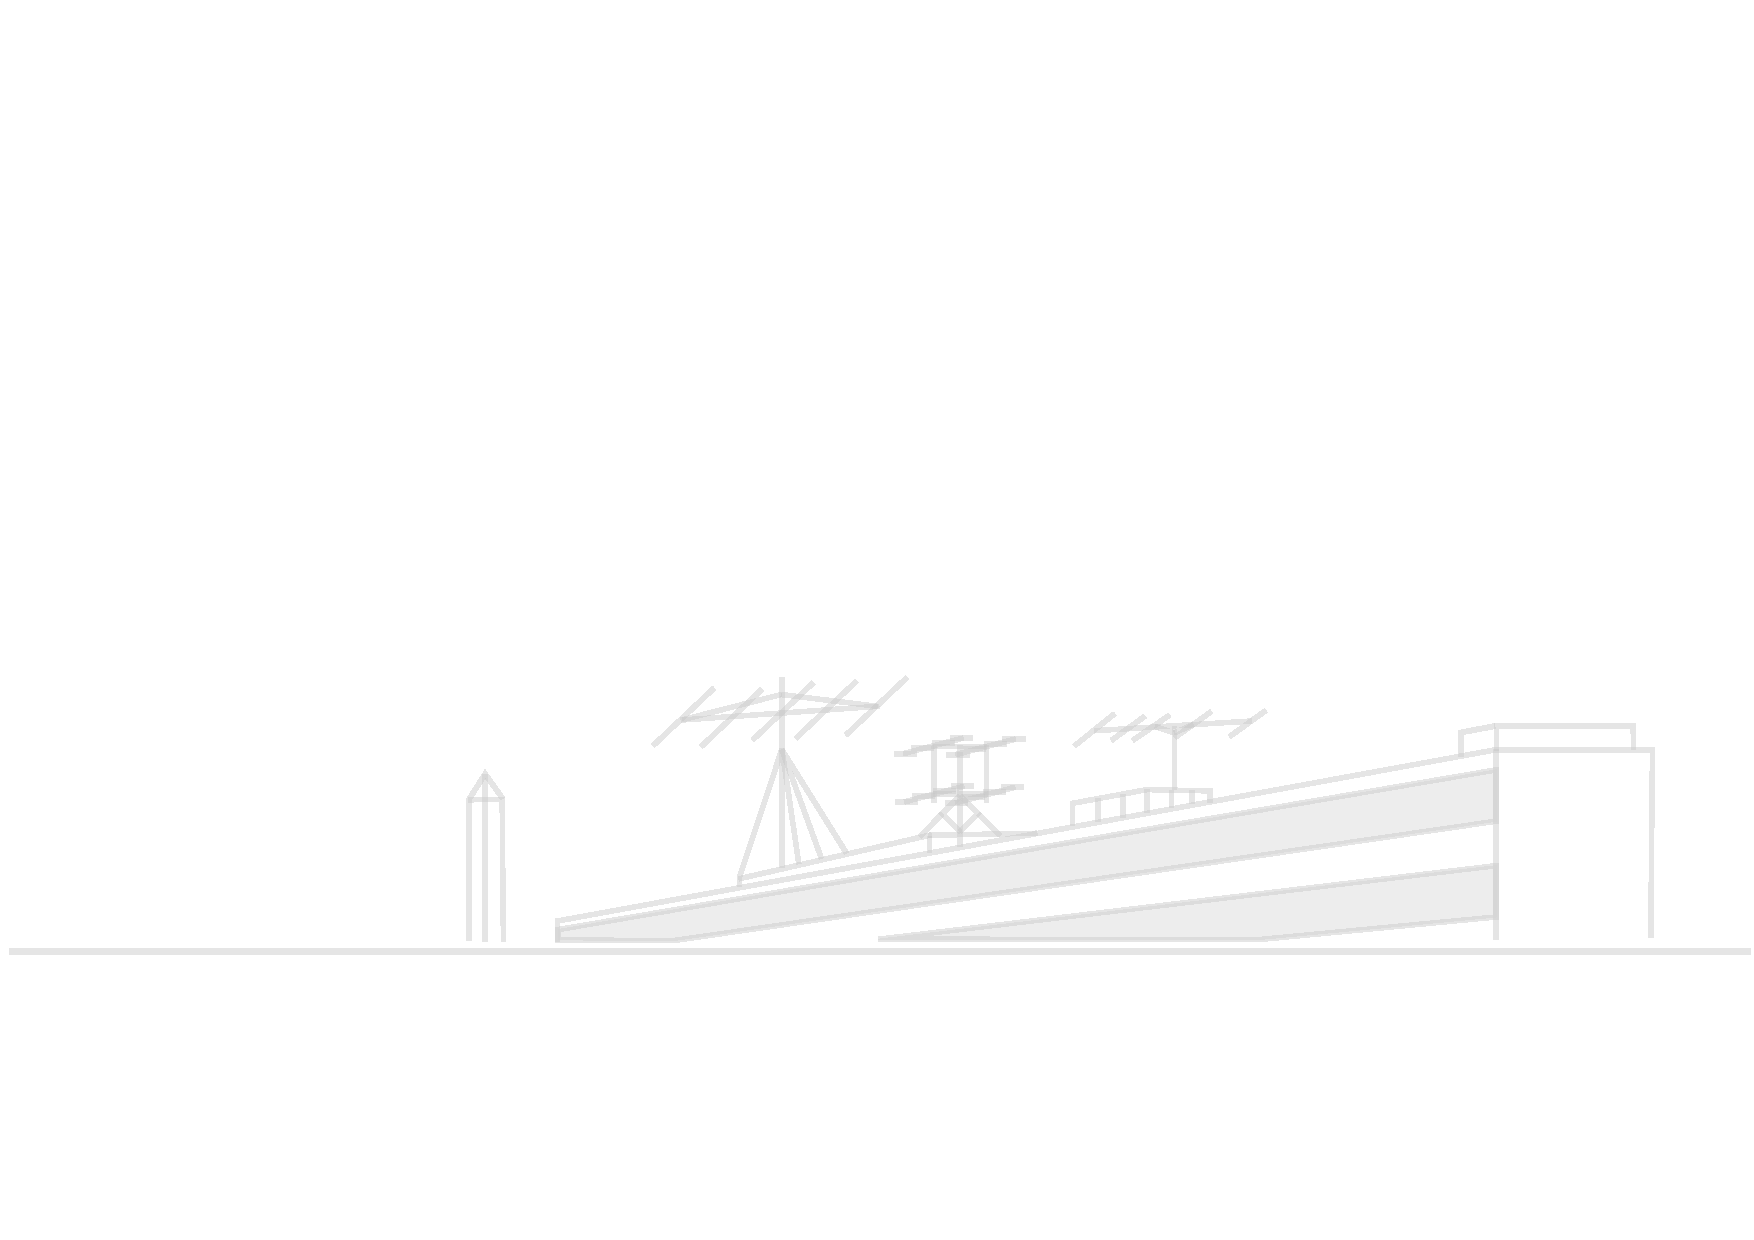
\includegraphics[width=17.8cm]{texdata/dk0tu_rooftop_background.pdf}
}

% Foliennummer einfügen
\setbeamertemplate{footline}[frame number]
%\setbeamertemplate{footline}{}

% Ändere das Zeichen vor jedem item
%\setbeamertemplate{itemize item}{\color{craneorange}$\blacktriangleright$}
%\setbeamertemplate{itemize subitem}{\color{craneorange}$\triangleright$}
%\setbeamertemplate{itemize subsubitem}{\color{craneorange}$\blacktriangleright$}

% Ändert die Blöcke 
\setbeamertemplate{blocks}[rounded][shadow=true]
% default | rounded [shadow=true|false]

%
% Eigene Kommandos
%

% Hack to get natbib and beamer working together. "The beamer user guide suggests
% that only the manual bibliography entry approach is supported"
% on some system it works out of the box, sometimes you need the hack :-(
% so check it --dl7bst
\ifdefined\newblock
    \relax
\else
    \newcommand{\newblock}{}
\fi

% \includedia command to generate png out of a dia file
% NEEDS installed dia and pdflatex option --shell-escape
\newcommand{\includedia}[1]{
    \immediate\write18{/usr/bin/dia #1.dia -e #1_diatmp.png -t png}
}

% RICHIG GROSSER FONT!
\newfont{\bigfont}{cmr10 at 144pt}
\newfont{\smallfont}{cmr10 at 8pt}

% Römische Ziffern
\makeatletter
\newcommand{\rmnum}[1]{\romannumeral #1}
\newcommand{\Rmnum}[1]{\expandafter\@slowromancap\romannumeral #1@}
\makeatother

% Schwarze Überschrift
%\setbeamercolor{frametitle}{fg=black}
%\setbeamercolor{title}{fg=black}

% Item- und Box-Farben
\definecolor{deepBlue}{HTML}{000066}
\setbeamercolor{itemize item}{fg=deepBlue}
\setbeamercolor{itemize subitem}{fg=deepBlue}
\setbeamercolor{description item}{fg=deepBlue}
\setbeamercolor{block title}{fg=deepBlue!100, bg=blue!15}
\setbeamercolor{block body}{fg=black, bg=blue!5}
\setbeamercolor{block title alerted}{fg=deepBlue, bg=red!75}
\setbeamercolor{block body alerted}{fg=black, bg=red!15}
\setbeamercolor*{block title example}{fg=blue!50, bg=blue!10}
\setbeamercolor*{block body example}{fg= blue, bg=blue!5}

%\setbeamercolor{section in head/foot}{parent=palette primary}
%\setbeamercolor{subsection in head/foot}{parent=palette secondary}
%\setbeamercolor{sidebar}{fg=darkblue,bg=yellow!90!orange}
%\setbeamercolor{title in sidebar}{fg=darkblue}
%\setbeamercolor{author in sidebar}{fg=darkblue}
%\setbeamercolor{section in sidebar}{fg=darkblue!10!black}
%\setbeamercolor{subsection in sidebar}{fg=darkblue!50!black}

% Titlepage Infos
\title{AFu-Kurs nach DJ4UF}
\author[DKØTU]{DKØTU\\ \footnotesize{Amateurfunkgruppe der TU Berlin}}
\institute[DKØTU]{\url{http://www.dk0tu.de} }

% PDF-Eigenschaften
\subject{DK0TU-Amateurfunkkurs nach DJ4UF}
\keywords{Amateurfunk Kurs HAM Radio Course CC-BY-NC-SA OpenSource TU Berlin DK0TU}

\subtitle{Betriebstechnik/Vorschriften 06: \\
  Rufzeichen - Landeskenner \\[2em]}
\date{Stand 31.10.2016}
 \begin{document}

\begin{frame}
    \titlepage
    \vfill
    \begin{center}
        \ccbyncsaeu\\
        {\tiny This work is licensed under the \em{Creative Commons Attribution-NonCommercial-ShareAlike 3.0 License}.}\\[0.5ex]
         \tiny Amateurfunkgruppe der Technische Universität Berlin (AfuTUB), DKØTU
         %\includegraphics[scale=0.5]{img/DK0TU_Logo.pdf}
    \end{center}
\end{frame}


% TODO keine langen TEXTE auf den Slides
% TODO Stumpf Listen vorlesen ist öde (Sind die roten Hervorhebungen auf dem Beamer erkennbar?)
% FIXME Ausschlussliste abgleichen und ggf verkleinern: http://www.funkwelle.com/amateurfunk/itu-landeskenner-lernen.html

\section{Einleitung}

\begin{frame}
  \frametitle{Einleitung / Disclaimer}

  \begin{center}
    \Large{Das Kapitel ist stark zusammengekürzt, da dieser Kurs eher
    praktischer Natur sein soll.}
  \end{center}

  \normalsize

  \begin{itemize}
    \item Es werden nur Landeskenner behandelt, die in Prüfungsfragen eine Rolle spielen.
    \item Zur Vollständigkeit lest bitte selbstständig die Lektion
      \texttt{B/V 06} im \emph{Moltrecht}!
  \end{itemize}

\end{frame}


\begin{frame}
  \frametitle{Einleitung / Rufzeichen}

  \begin{center}
    \Large{Wozu gibt es Rufzeichen?} \\[1em]
    \Large{Welche kennt ihr bereits und wie unterscheiden sie sich? ($\Rightarrow$~Tafel)}
  \end{center}

\end{frame}

%\begin{frame}
%    \frametitle{Einleitung / Landeskenner}
%
%    \begin{center}
%        \Large{Landeskenner im Präfix -}
%        Wurde vermutlich schon erkannt.
%    \end{center}
%
%\end{frame}

\section{Rufzeichen}

\begin{frame}
  \frametitle{Rufzeichen}

  In \textbf{DL} personengebunden. Kann aber in anderen Staaten auch an die Station
  gebunden sein. \\[1em]

  Mindestens drei, normalerweise bis sechs Zeichen. Kann aber auch länger
  sein.\footnote{\scriptsize Ausnahme: Sonder-Calls, z.B.
  \texttt{DL65DARC} oder \texttt{DG500BIER}}

\end{frame}

\begin{frame}[fragile]
  \frametitle{Rufzeichen}

  Aufbau:

  \begin{itemize}
    \item 2-3 Zeichen \textbf{Präfix}
      \begin{itemize}
        \item 1-2 Zeichen Landeskenner
        \item 1 Ziffer (z.B. Lizenzklasse, Region, ...)
      \end{itemize}
    \item $>$1 Zeichen \textbf{Suffix}
  \end{itemize}

  \pause

  \begin{block}{Regular Expression}
    \verb+/^([A-Z0-9]{1,2})([0-9]{1})([A-Z]{1,3})$/+
  \end{block}


\end{frame}

\section{Landeskenner}

\begin{frame}
  \frametitle{Landeskenner}

  \begin{center}
    Deutschland: D\textbf{A}--D\textbf{R} \\[1em]
  \end{center}

  Vorsicht! \\
  DS--DT: Südkorea \\
  DU--DZ: Philippinen \\[1em]

\end{frame}

\begin{frame}
  \frametitle{Landeskenner}

  Nachschlagewerke für Landeskenner:

  \begin{itemize}
    \item ITU (Appendix 42 to the RR)
      \footnote{\scriptsize\ExternalLink\url{http://www.itu.int/online/mms/glad/cga_callsign.sh?lng=E}}
    \item DXCC Entities List\footnote{\scriptsize\ExternalLink\url{http://www.arrl.org/country-lists-prefixes}}
      (Landeskennerliste) der ITU
    \item Amateurfunkhandbücher
    \item Rufzeichenlisten
    \item ausführliche Präfixlisten\footnote{\scriptsize z.B. \ExternalLink\url{http://ac6v.com/prefixes.htm}}
      (genauer unterteilt als nur Landeskenner)
    \item Logging Software
  \end{itemize}

\end{frame}

\begin{frame}
  \frametitle{Landeskenner}

  Folgende Listen sind nicht vollständig
  $\rightarrow$ nur in den Prüfungsaufgaben genannte \\[3em]

  \alert{Rot hervorgehobene Länder lernen} für Ausschlussverfahren

\end{frame}

\subsection{Europäische Landeskenner}

%    Don't Panic! ''Eselsbrücken'' helfen weiter, z.B.:

\begin{frame}
  \frametitle{Europäische Landeskenner}

  \begin{tabular}{l|l|l}
    Kenner & Land & Eselsbrücke\\ \hline
    C3 & Andorra & \\
    CT & Portugal & \\
    \alert<2>{DL (DA\ldots DR)} & \alert<2>{Deutschland} & \\
    \alert<2>{EA (EB, EC, ED)} & \alert<2>{Spanien} & \textbf{E}spañ\textbf{a} \\
    \alert<2>{EI} & \alert<2>{Irland} & \textbf{Ei}re \\
    EM (UT) & Ukraine & \\
    \alert<2>{ES} & \alert<2>{Estland} & \\
    \alert<2>{F} (FA\ldots FE) & \alert<2>{Frankreich} & \\
    G (GB\ldots GM, M) & Großbritannien & \\
    GM (MM) & Schottland & \\
    HA & Ungarn & \textbf{H}ung\textbf{a}ry\\
    \alert<2>{HB, HB9} & \alert<2>{Schweiz} & \textbf{H}ohe \textbf{B}erge (\textbf{H}elvetia) \\
    \alert<2>{HB\O} & \alert<2>{Liechtenstein} & \\
    HV & Vatikan & \textbf{H}eiliger \textbf{V}ater \\
  \end{tabular}

\end{frame}

\begin{frame}
  \frametitle{Europäische Landeskenner}

  \begin{tabular}{l|l|l}
    Kenner & Land & Eselsbrücke\\ \hline
    I (IA\ldots IZ) & Italien & \\
    \alert<2>{LA} (LB) & \alert<2>{Norwegen} & \textbf{La}chse \\
    \alert<2>{LX} & \alert<2>{Luxemburg} & \textbf{L}u\textbf{x}emburg \\
    LY & Litauen & \\
    \alert<2>{LZ} & \alert<2>{Bulgarien} & \\
    OE & Österreich & \\
    \alert<2>{OH} & \alert<2>{Finnland} & \\
    OK & Tschechien & \\
    OM & Slowakei & \\
    \alert<2>{ON} & \alert<2>{Belgien} & \\
    OY & Faröer Inseln & \\
    \alert<2>{OZ} & \alert<2>{Dänemark} & \\
    \alert<2>{PA} (PB, PD, PE, PI) & \alert<2>{Niederlande} & \textbf{Pa}ys-Bas \\
    UA (RA\ldots) & Russland & \\
  \end{tabular}

\end{frame}

\begin{frame}
  \frametitle{Europäische Landeskenner}

  \begin{tabular}{l|l|l}
    Kenner & Land & Eselsbrücke\\ \hline
    SM & Schweden & \\
    \alert<2>{SP} & \alert<2>{Polen} & \textbf{S}chönes/\textbf{S}oz. \textbf{P}olen \\
    SV & Griechenland & \\
    \alert<2>{S5} & \alert<2>{Slowenien} & \\
    TA & Türkei & \\
    \alert<2>{YL} & \alert<2>{Lettland} & \textbf{Y}oung \textbf{L}atvian \\
    \alert<2>{YO} & \alert<2>{Rumänien} & \\
    YU & Serbien & \\
    \alert<2>{3A} & \alert<2>{Monaco} & \\
    \alert<2>{4U} & \alert<2>{Vereinte Nationen} & For You \\
    \alert<2>{9A} & \alert<2>{Kroatien} & \\
    \alert<2>{9H} & \alert<2>{Malta} & \\
  \end{tabular}
\end{frame}

%\begin{frame}
%  \frametitle{Übung}
%  \begin{center}
%    \begin{tabular}{l||p{.8\textwidth}}\hline
%      \textbf{BD206} & \textbf{Welche Länder sind der Reihe nach den folgenden Landeskennern zugeordnet? Die Landeskenner OE, OH, OK, OM, ON, OZ entsprechen den Ländern} \\\hline\hline
%      A & Österreich, Belgien, Tschechien, Slowakei, Finnland, Dänemark. \\ \hline
%      B \only<2>\checkmark & Österreich, Finnland, Tschechien, Slowakei, Belgien, Dänemark. \\ \hline
%      C & Österreich, Finnland, Tschechien, Belgien, Slowakei, Dänemark. \\\hline
%      D & Österreich, Slowakei, Tschechien, Finnland, Belgien, Dänemark. \\\hline
%    \end{tabular}
%  \end{center}
%\end{frame}
%
%\begin{frame}
%  \frametitle{Übung}
%  \begin{center}
%    \begin{tabular}{l||p{.8\textwidth}}\hline
%      \textbf{BD202} & \textbf{Welche Gruppe von Ländern grenzt an die Bundesrepublik Deutschland?} \\\hline\hline
%      A & SM, LA, LZ, HB \\ \hline
%      B & EA, GM, OE, ON \\\hline
%      C \only<2>\checkmark & F, HB, OZ, SP \\ \hline
%      D & CT, I, LX, OK \\\hline
%    \end{tabular}
%  \end{center}
%\end{frame}

\subsection{Außereuropäische Landeskenner}

\begin{frame}
  \frametitle{Außereuropäische Landeskenner: RR Funkregionen}

  \begin{center}
    \begin{figure}
      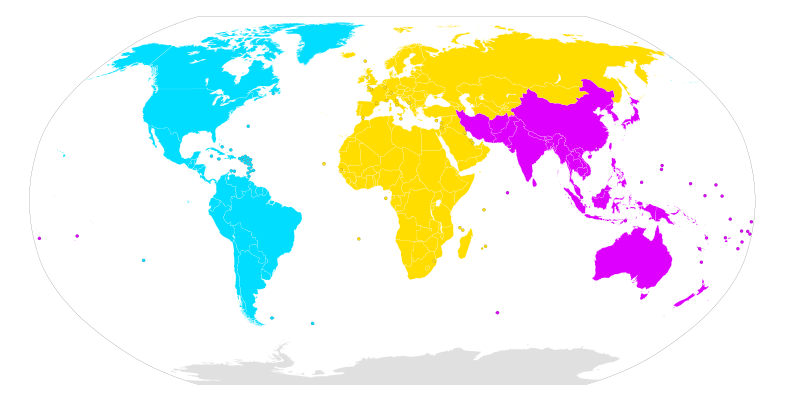
\includegraphics[width=.7\textheight]{bv06/International_Telecommunication_Union_region-800px.png}
      \attribcaption{A map of the world divided into International Telecommunication Union regions}{BlankMap-World6.svg: Canuckguy (talk) and many others derivative work: Denelson83 (BlankMap-World6.svg)}{https://commons.wikimedia.org/wiki/File:International_Telecommunication_Union_region.svg}{\ccpd}
    \end{figure}
  \end{center}

  \small{
  \begin{description}
    \item[Region 1] Europa, Afrika, Vorderasien (ohne Iran), Russland, Georgien,
      Armenien, Aserbaidschan, Kasachstan, Turkmenistan,
      Usbekistan, Tadschikistan, Kirgisistan, Mongolei
    \item[Region 2] Nord- und Südamerika, Karibik, Grönland, Hawaii
    \item[Region 3] Australien, Neuseeland, Ozeanien und Asien ohne die unter
      Region~1 genannten Länder Asiens.
  \end{description}
  }

\end{frame}

\begin{frame}
  \frametitle{Außereuropäische Landeskenner: Region 1}

  In der Prüfung genannt\hspace{2pc}\only<2>{\alert{Lernen für Ausschlussverfahren}}\\[1em]

  \begin{tabular}{l|l|l}
    Kenner & Land & Eselsbrücke\\ \hline
    \alert<2>{3V} & \alert<2>{Tunesien} & \\
    5N & Nigeria &  \\
    4X & Israel & \\
    5B & Zypern & \\
    5H & Tansania & \\
    9X & Ruanda & \\
    EL & Libera & \\
    ST & Sudan & \\
    \alert<2>{SU} & \alert<2>{Ägypten} & \textbf{Su}eskanal \\
    UA9, UA0 & asiatisch Russland & \\
    YK & Syrien & \\
    ZS & Südafrika & \\
  \end{tabular}

\end{frame}

\begin{frame}
  \frametitle{Außereuropäische Landeskenner: Region 2}

  In der Prüfung genannt\hspace{2pc}\only<2>{\alert{Lernen für Ausschlussverfahren}}\\[1em]

  \begin{tabular}{l|l|l}
    Kenner & Land & Eselsbrücke\\ \hline
    CE & Chile &  \\
    \alert<2>{HC} & \alert<2>{Ecuador} & \\
    \alert<2>{HK} & \alert<2>{Kolumbien} & \\
    \alert<2>{K, W, N, A} & \alert<2>{USA} & \textbf{K}einer \textbf{W}ill \textbf{N}ach \textbf{A}merika\\
    \alert<2>{LU} & \alert<2>{Argentinien} & \textbf{L}inks \textbf{U}nten \\
    \alert<2>{OA} & \alert<2>{Peru} & \textbf{O}st-\textbf{A}nden \\
    \alert<2>{PY} & \alert<2>{Brasilien} & \textbf{P}iranha \\
    \alert<2>{VE} & \alert<2>{Kanada} & \textbf{V}iele \textbf{E}lche \\
    XE, XF & Mexiko & \\
    \alert<2>{YV} & \alert<2>{Venezuela} & \\
  \end{tabular}

\end{frame}

\begin{frame}
  \frametitle{Außereuropäische Landeskenner: Region 3}

  In der Prüfung genannt\hspace{2pc}\only<2>{\alert{Lernen für Ausschlussverfahren}}\\[1em]

  \begin{tabular}{l|l|l}
    Kenner & Land & Eselsbrücke\\ \hline
    BV & Taiwan & \\
    \alert<2>{BY} & \alert<2>{China} & \textbf{B}uy \textbf{$\text{\yen}$}uan \\
    DS\ldots DT & Südokorea & \\
    DU\ldots DZ & Philippinen & \\
    EP & Iran & \\
    \alert<2>{JA}, JE\ldots JS & \alert<2>{Japan} & \\
    JT & Mongolei &  \\
    VK & Australien & \textbf{V}iele \textbf{K}ängurus \\
    VU & Indien & \\
    \alert<2>{ZL} & \alert<2>{Neuseeland} & \textbf{Z}ea\textbf{l}and\\
    4S & Sri Lanka &  \\
  \end{tabular}

\end{frame}

\section{T/R 61-01}

\begin{frame}
  \frametitle{CEPT-Empfehlung T/R 61-01}

  Wenn die Empfehlung vom Staat anerkannt wird\footnote{aktuell 52 Staaten
  \ExternalLink\url{http://www.darc.de/fileadmin/filemounts/referate/ausland/CEPT-Laenderliste_2015.pdf}}, darf
  man mit einem zusätzlichen Präfix vorübergehend Amateurfunk ausüben.
  Beispiele:

  \begin{itemize}
    \item \textbf{F/}DL7BST
    \item \textbf{DL/}HB9ZZ
    \item ...
  \end{itemize}

  Mehr dazu in der Lektion \texttt{BV07}.

\end{frame}

\section{Zusatz-Kenn\-zeich\-nungen}

\begin{frame}
  \frametitle{Zusatz-Kennzeichnungen}

  Es ist möglich, aber nicht zwingend notwendig, folgende
  Zusatz-Kennzeichnungen beim Funkbetrieb zu verwenden:

  \begin{description}
    \item[/p] \textit{portable} vorübergehender ortsfester Funkbetrieb
    \item[/m] \textit{mobile} bewegliche Amateurfunkstellen, z.B. KFZ, Fahrrad, Boot (Binnengewässer)
    \item[/mm] \textit{maritime mobile} offene See (kein Binnengewässer!)
    \item[/am] \textit{aeronautic mobile} Luftfahrzeug
  \end{description}

  Eine Sondergenehmigung ist für all diese Betriebsarten nicht notwendig. Auch
  laut \emph{StVO} ist Funken am Steuer nicht verboten.

\end{frame}

\section{Deutsche Rufzeichen}

\begin{frame}
  \frametitle{Deutsche Rufzeichen}

  Geregelt im \textbf{Rufzeichenplan gemäß § 10 Abs. 3 AFuV}. \\[1em]

  In diesem finden sich alle zugeteilten Rufzeichen in Verbindung mit dem
  Namen des Inhabers und die Standorte von Relaisfunkstellen und Funkbaken.
  \\[1em]

  Inzwischen auch online\footnote{\scriptsize\ExternalLink\url{http://ans.bundesnetzagentur.de/Amateurfunk/Rufzeichen.aspx}}
  abrufbar.

  %todo Aufteilung DL Rufzeichen siehe Moltrecht.

  Ausführliche Liste der deutschen Rufzeichenblöcke in der Wikipedia
  \footnote{\scriptsize\ExternalLink\url{http://de.wikipedia.org/wiki/Amateurfunkrufzeichen}}. \\[1em]

  Einzige Prüfungsfrage: Zuordnung des Präfix \textbf{DO}.

\end{frame}

\section{Lernhinweise}

\begin{frame}
  \frametitle{Lernhinweise}

  \begin{itemize}
    \item zeitnah die Moltrecht-Lektion \texttt{B/V 06} durcharbeiten
    \item in der Prüfung geht es vorrangig um die europäischen und einige
      außereuropäische Landeskenner, die reduziert werden können
    \item Eselsbrücken
    \item Ausschlussverfahren
      \ldots noch geschicktere Ausschlussverfahren (rote Rufzeichen in den Listen)
    \item nicht fertig machen lassen und in der Woche vor der Prüfung
      nochmal alles mit dem Simulator durchklicken
  \end{itemize}

\end{frame}

%\begin{frame}
%  \begin{alertblock}{Hausaufgabe}
%    Die Aufgaben zu Rufzeichen und Landeskenner durcharbeiten: Prüfungfragen ``Betriebliche Kenntnisse'' Kapitel 2.4 ``Rufzeichen, Landeskenner'' mit ``Deutsche Rufzeichen'' (BD101--BD115), ``Europäische Landeskenner'' (BD201--BD210) und ``Internationale Landeskenner'' (BD301--BD309).
%  \end{alertblock}
%\end{frame}

\renewcommand{\refname}{Referenzen}

\hypertarget{refs}{}
\textcolor{white}{} \\ %\vspace{} geht nicht
\Large Referenzen/Links
\footnotesize

\begin{thebibliography}{}
  \bibitem{darc}  DARC Online-Lehrgang Lektion B/V 06: \\
    \url{http://www.darc.de/der-club/referate/ajw/lehrgang-bv/bv06/}
  \bibitem{wp}    Wikipedia - Die freie Enzyklopädie: \\
    \url{http://de.wikipedia.org/wiki/Amateurfunkrufzeichen} \\
    \url{http://de.wikipedia.org/wiki/Regelungen_im_Amateurfunkdienst}
\end{thebibliography}

% Hier könnte noch eine Kontaktfolie stehen

\end{document}

